\documentclass[a4paper, 12pt,oneside]{article} 
%\documentclass[a4paper, 12pt,oneside,draft]{article} 
\usepackage{preamble}
%--------------------- ACTUAL FILE ---------------------- %
\begin{document} 
%%%
	\begin{titlepage}
    \newcommand{\HRule}{\rule{\linewidth}{0.5mm}} % Defines a new command for the horizontal lines, change thickness here
    
    \center  % Center everything on the page
     
    %----------------------------------------------------------------------------------------
    %   HEADING SECTIONS
    %----------------------------------------------------------------------------------------

    \vspace{3cm}
    \textsc{\LARGE École polytechnique fédérale de Lausanne}\\[1.5cm] % Name of your university/college
    
    \textsc{\Large Regression Methods Project Report}\\[0.5cm] % Major heading such as course name
    \textsc{\large Coin-Data Regression Study}\\[0.5cm] % Minor heading such as course title
    
    %----------------------------------------------------------------------------------------
    %   TITLE SECTION
    %----------------------------------------------------------------------------------------
    
    \HRule \\[0.4cm] % line above and under the title
    
    
    % Title of your document
    
    \HRule \\[1.5cm]
     
    %----------------------------------------------------------------------------------------
    %   AUTHOR SECTION
    %----------------------------------------------------------------------------------------
    
    \begin{minipage}{0.4\textwidth}
    \begin{flushleft} \large
    
    \emph{Authors:}\\
    Tara \textsc{Fjellman}\\
    Rayan \textsc{Harfouche}\\
    
    
    
    
    \end{flushleft}
    \end{minipage}
    ~
    \begin{minipage}{0.4\textwidth}
    \begin{flushright} \large
    
    \emph{Professor:} \\
    Anthony \textsc{Davison}\\
    \end{flushright}
    \end{minipage}\\[10cm]
    %
    
    
    %----------------------------------------------------------------------------------------
    %   LOGO SECTION
    %----------------------------------------------------------------------------------------
    
    
\includegraphics[width=0.4\linewidth]{Logo-1 .pdf}\\[1cm] 
    % Include a department/university logo - this will require the graphicx package
     
    %----------------------------------------------------------------------------------------
    
    \vfill % Fill the rest of the page with whitespace
    
    \end{titlepage} 
	% Add titlepage
	\clearpage
	\tableofcontents
	\thispagestyle{empty}
	\vspace{2cm}
	\section*{Abstract}
		context of the original paper (with their claims). The paper that won the 2024 IgNobel Prize in Probability took a Bayesian approach to studying the statistics behind the coin-flipping process. Its main goal was to confirm a prediction made by a physical model of human coin tossing developed by Diaconis, Holmes, and Montgomery (DHM; 2007); i.e. that when people flip an ordinary coin, the probability of it landing on the same side it started is about 51\%. 
		It also revealed considerable between-people variation in the degree of this same-side bias, as well as its decrease as more coins were flipped. 

		The goal of this report is two fold. On the one side, we aim to investigate similar questions with a regression approach : 
		is there evidence for between-person, between-coin, or even person-coin pair differences ? To what extent does flipping experience affect the observed same-side bias ?
		In addition, we also investigate the differences between GLM and WLS approaches; as well as muscle memory effects (through outcomes of recent flips). 
		\begin{itemize}
			\item add more interpretation of models ?? 
			\item work on abstract
			\item derive conclusion from abstract 
			\item discussion for glm model comparison
			\item clean/delete irrelevant code-cells/files
			\item ....
		\end{itemize}
	\clearpage
	\pagenumbering{arabic}
	\setcounter{page}{1}
	\section{Introduction}
		Before diving into the analysis, we provide a brief overview of the datasets' main features and the models we consider. Our exploratory analysis is available as a Jupyter notebook, and provides more detail as well as the plots supporting our claims.

		The dataset is composed of throws from 48 people using 44 coin types in total. Given the study did not impose strict guidelines for coins to be used, the design is heavily unbalanced. Eighteen coins have only been thrown by a single person, while some of them have been thrown by more than 20 people. Also, around two-thirds of the people have only flipped 5 or fewer different coins, while someone threw 11 different ones. As for the the person-coin pairs, most have 1000 throws or fewer, while some have around 10000. This severe unbalance must be kept in mind during the analysis, given it restricts the methods that can be used and poses challenges during model interpretation. 

		After plotting the same-side proportion across people, coin and person-coin combinations, we deemed it relevant to investigate models considering both person and coin as covariates, as well as individual person-coin pairs. Following the advice given on the project statement, we also branched our analysis in binomial-response GLM and WLS approaches, with the goal of comparing the results. 

		Motivated by impacts of muscle-memory on the flipping, we additionally investigated time-varying same-side proportions and memory between successive throws.
	\section{Analysis}
		\subsection{Model Comparison}
			In this section, we introduce and compare different models for the same-side proportion. 

			Before thinking about models, we thought about whether transforming the response was relevant. Given the same-side rates where clustered around 50\% with little change around it, we did not see any reason a priori to apply a transformation to the response. Diagnostic plots were of course later inspected to confirm this intuition.
			
			As for the covariates we considered in our models, we of course included the person throwing and the coin being thrown as categorical covariates. Due to the potential we saw in time-effects to alias with coin effects (explanations will come in \ref{sec:disc-learning-effects}), we preferred including time in this analysis instead of relegating it to an independent part. This was done by considering the version of the data that is composed of ordered sequences/entries of 100 (or so) throws at a time for a fixed person-coin combination. Considering this data also allowed us to try and estimate effects of coins nested within people, trying to capture subjectivity in how people perceive given coins. Indeed, doing this on the aggregated data would have yielded a saturated model. 

			In the next section, we start by introducing the theory on which we base our model selection. 
			\subsubsection{Tools For Selection}
				Following the suggestion in the project statement, we compare candidate models both with help of Akaike's Information Criterion (AIC) and Likelihood Ratio Tests (LRTs). 

				We recall that AIC is defined as 
				\begin{gather}
					\text{AIC}:=2p-2\ln\left(\sup_{\theta\in\Theta}\mathcal{L(\theta)}\right),
				\end{gather}
				with $p$ the number of degrees of freedom of the model, $\mathcal L$ is the likelihood function for the model, and $\Theta$ is the parameter space. By minimising AIC over candidate models, one is therefore rewarding model fit, while penalising by a $2p$ term to avoid overfitting. Its goal is therefore to yield parsimonious predictive models. It does not make any assumption about compared models being of similar interpretation or nested. 

				In contrast, LRT is specifically designed for comparing a model $A$ with a nested (or restricted) one $B$. It is based on the fact that 
				\begin{gather}
					\lambda_{LR}:=-2\ln\left[\frac{\sup_{\theta\in\Theta_B}\mathcal{L(\theta)}}{\sup_{\theta\in\Theta_A}\mathcal{L(\theta)}}\right]
					\overset{H_0}{\sim} \chi^2_{p_A-p_B},
				\end{gather}
				where $\Theta_A\supset\Theta_B$ respectively are the parameters spaces (of dimension $p_a>p_b$) associated to models $A$ and $B$, and $H_0$ is the null hypothesis : the true optimal $\theta$ is in $\Theta_B$. Given this definition, LRTs are used to shed light on whether extra degrees of freedom improve the model significantly better than chance. This has applications in explanatory models, but might be of limited use in the context of model selection due to being prone to overfitting. This is particularly true when testing many models, as tests become correlated and give rise to spurious results (see slide 138 of [2]).

				Note that both differences of AIC and LRTs are tools that are often formulated in terms of difference of deviances associated to the models
				\begin{gather}
					\lambda_{LR} = 2\ln \sup_{\theta\in\Theta_A}\mathcal{L(\theta)} - 2 \sup_{\theta\in\Theta_B}\mathcal{L(\theta)} = D_B-D_A,\\
					\Delta \text{AIC} = \text{AIC}_A - \text{AIC}_B = 2(p_A-p_B) - (D_B-D_A). 
				\end{gather}
			\subsubsection{Diagnostic Plots}
				To asses the quality of the models, the diagnostics we decided to use are 
				\begin{itemize}
					\item A QQ plot to check normality of normalised residuals. Pearson studentized residuals were used for WLS models while the $r_j^*=r_{D j}+r_{D j}^{-1} \log \left(r_{P j} / r_{D j}\right) \dot{\sim} N(0,1)$ residuals were used for GLM models (where $r_{P j},r_{D j}$ refer to normalised versions of Pearson and deviance residuals). Normality corresponds to a roughly straight line, while outliers, skewness and heavy tails are easily spotted as deviations from it.
					\item A scatter plot of residuals as a function of fitted values, to assess linearity and homoscedasticity. Pearson studentized residuals were used for WLS models, while deviance residuals were used for GLM models. Linearity corresponds to residuals that stay centred around 0 across the fitted values, while homoscedasticity corresponds to residuals whose spread is constant across the fitted values.
					\item Cook's distance as a function of data index to reveal highly influential data points. Points over the $8/(n-2p)$ threshold are given a closer look (in order of importance). 
					\item Scatter plots (resp. box-plots for categorical covariates) of Pearson residuals as a function of the covariates of interest. These are used to check for independence between residuals and the covariates. If there is independence, the residuals look uncorrelated with respect to the covariates. 
				\end{itemize}
				These choices were motivated by our understanding of section 1.4 of [2]. 
			\subsubsection{WLS Approach}
			In this section, we consider the normal approximation for the binomial variable $R$ (the same-side flips within a sequence) with denominator $m$ (number of flips within a sequence). 
			Having that the success probability is fairly close to 0.5 we get $p(1-p)\approx1/4$. Hence we end up with the approximation $R/m \sim N(p,1/(4m))$. 
			\begin{table}[htb]
				\centering
				% Top subtable
				\begin{subtable}{\textwidth}
					\centering
					\caption{ANOVA (type II) of the WLS \texttt{1+person+agg+coin+person:coin} model and AIC values of cumulative terms.}
					\label{tab:WLS-AIC}
					\begin{tabular}{lccccc}
					\toprule
					Term & RSS & df & F & P($\ge F$) & AIC \\
					\midrule
					\texttt{1} & - & - & - & - & 159.76  \\
					\texttt{person} & 213.78 & 46.00 & 4.31 & 4.47e-20 & 12.89 \\
					\texttt{agg} & 7.65 & 1.00 & 7.10 & 7.75e-03 & 0.00 \\
					\texttt{coin} & 57.95 & 42.00 & 1.28 & 1.07e-01 & 29.21 \\
					\texttt{Residual} & 3576.62 & 3319.00 & - & - & 0.00 \\
					\bottomrule
					\end{tabular}
				\end{subtable}
				%\vspace{1em} % Optional vertical spacing

				\begin{subtable}{\textwidth}
					\centering
					\caption{LRTs for the WLS fitted models.}
					\label{tab:WLS-LRT}
					\begin{tabular}{lcc}
					\toprule
					Tested model & Restricted Model & p-value \\
					\midrule
					\texttt{1 + C(person)} & \texttt{1} & 0.00 \\
					\texttt{1 + C(person) + agg} & \texttt{1 + C(person)} & 0.00 \\
					\texttt{1 + C(person) + agg + C(coin)} & \texttt{1 + C(person) + agg} & 0.09 \\
					\texttt{1 + C(person) + agg + C(person):C(coin)} & \texttt{1 + C(person) + agg} & 0.02 \\
					\bottomrule
					\end{tabular}
				\end{subtable}
				%\caption{Main caption for the stacked tables.}
				%\label{tab:stacked_tables}
			\end{table}	

			[TABLES STILL HAVE C(PERSON) ETC, removing spaces between symbols can also make table more concise, no ?] We fit a linear model using weighted least squares, where the  weight associated to each entry is proportional to the inverse of the variance, that only depends on $m$. As the weights are only relevant up to a common factor, we normalise them by the average of the weights of all the entries. This does not change the result of the regression. 
			\begin{figure}[h!]
				\centering
				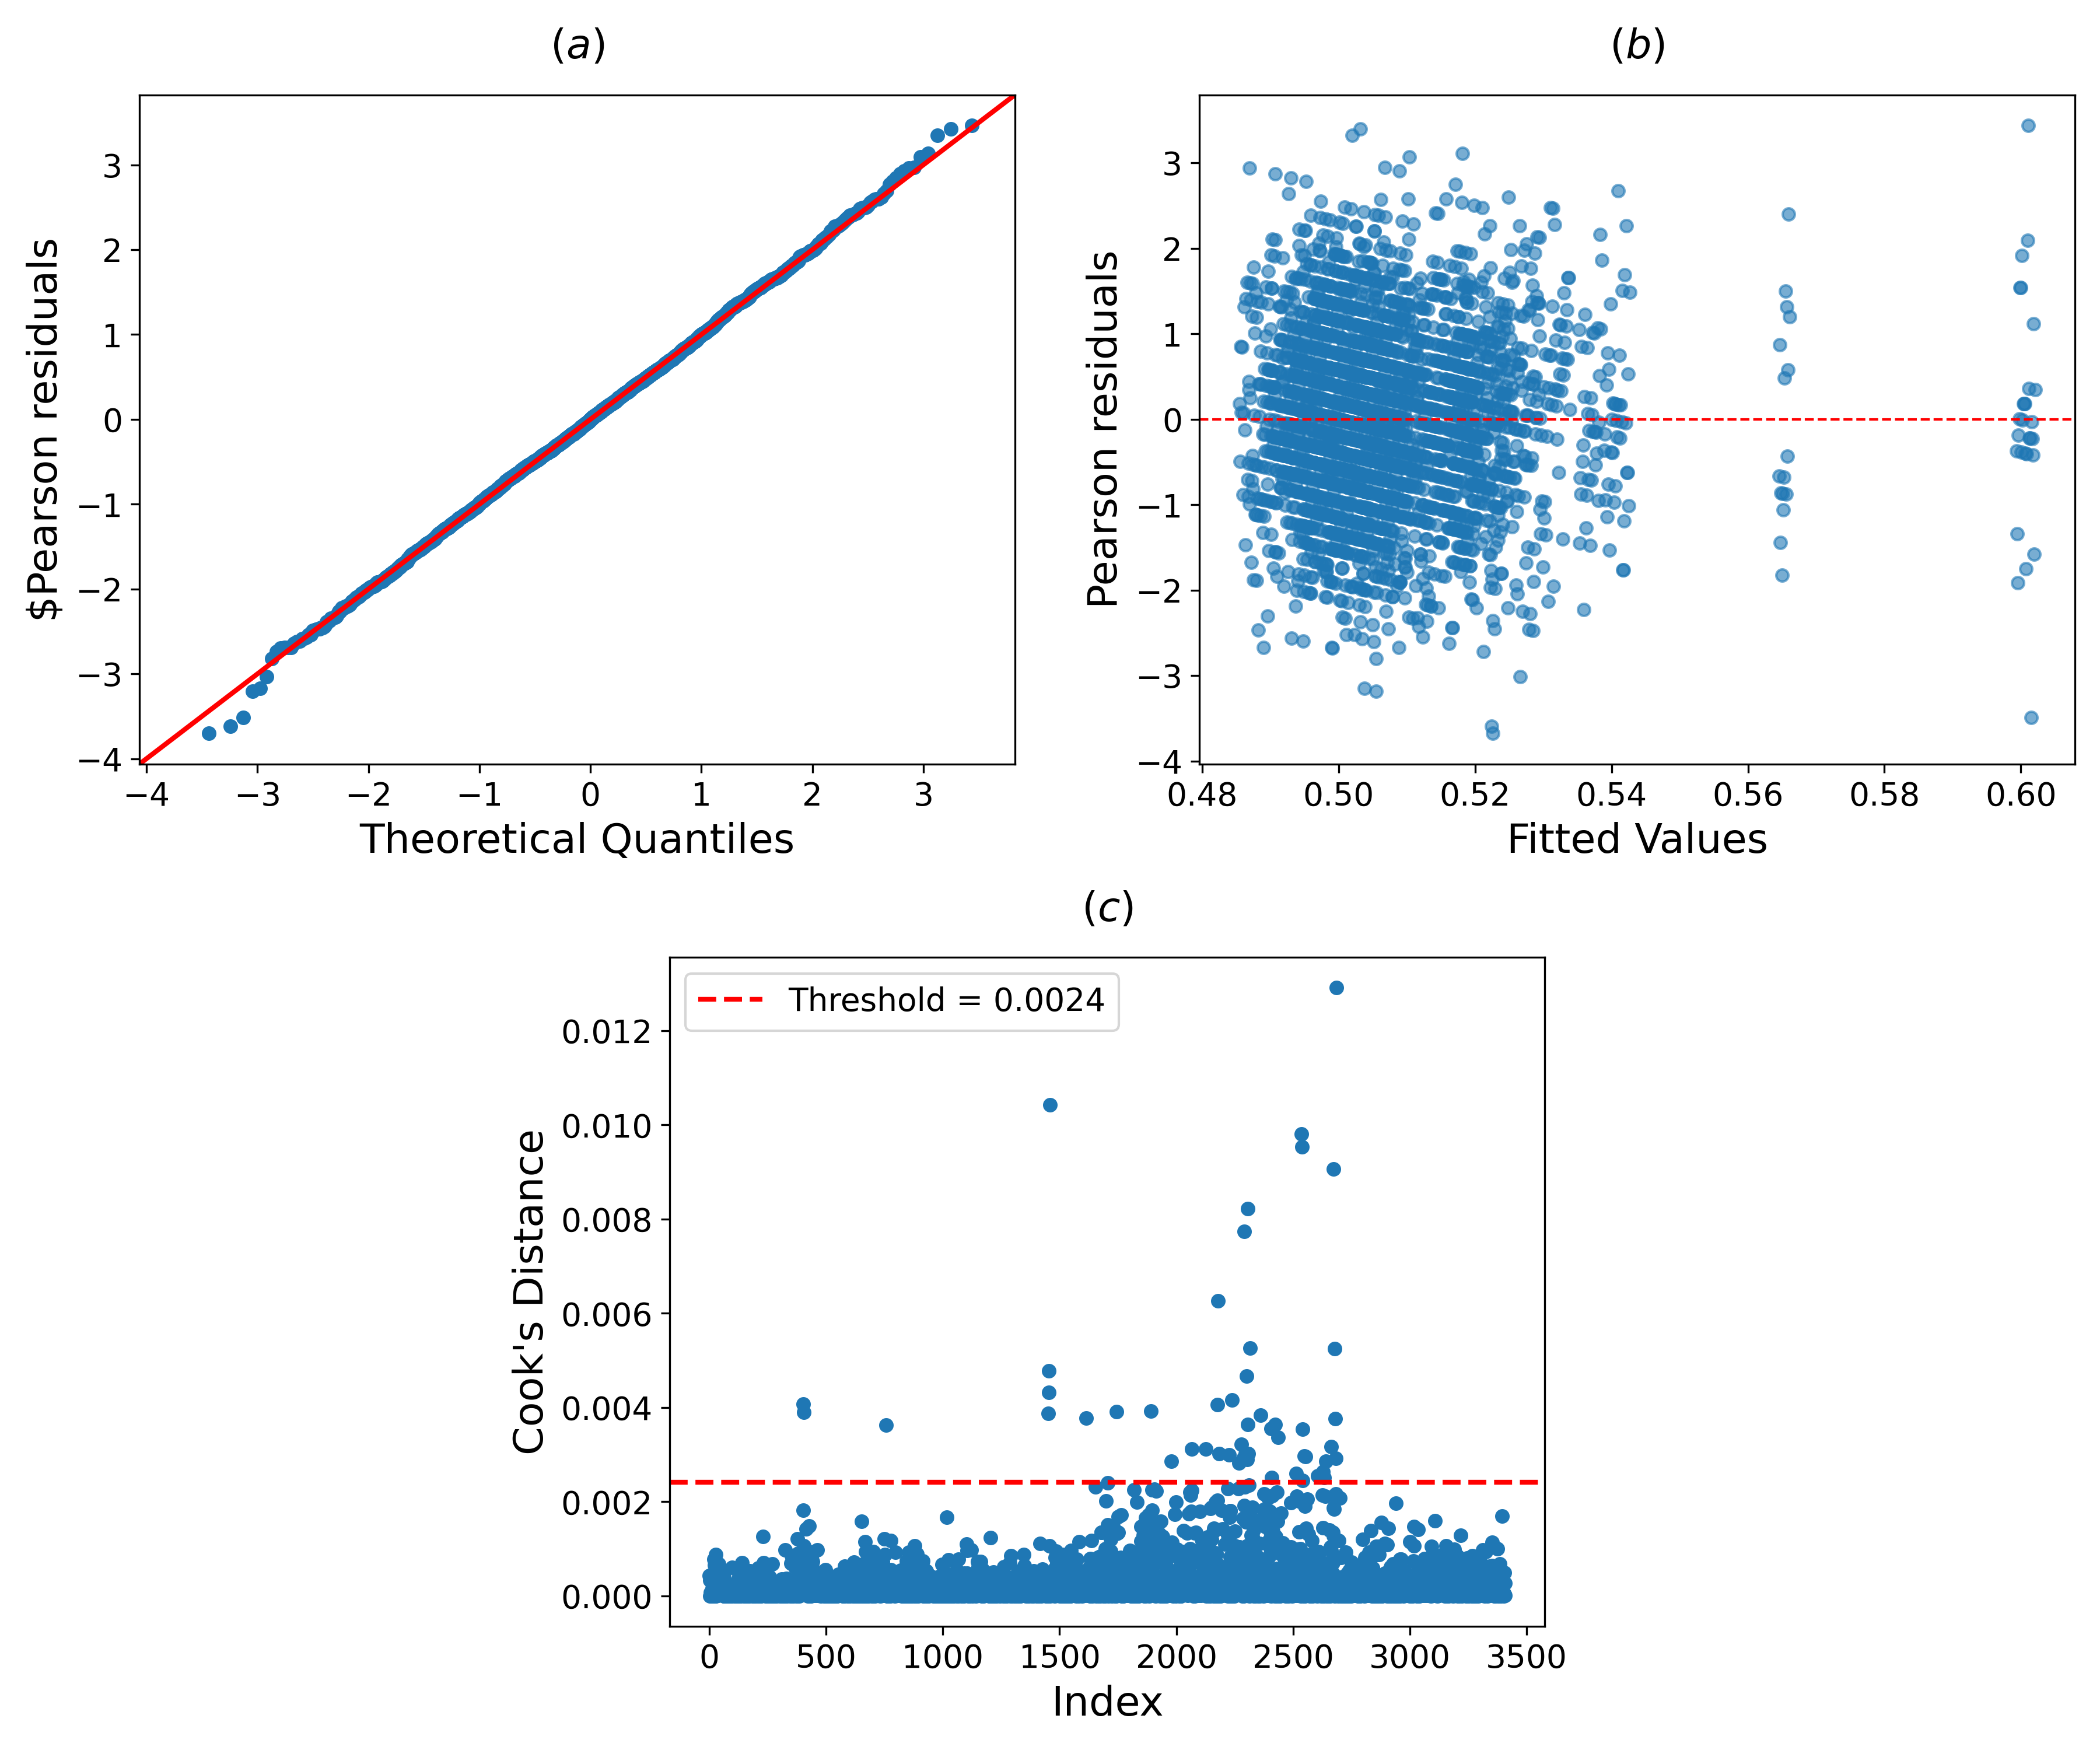
\includegraphics[width=0.8\textwidth]{WLS_diagnostics.png}
				\caption{Main diagnostics for the WLS \texttt{1+person+agg} model.}
				\label{fig:wls-diagnostic}
			\end{figure}
			
			[FOR THE WLS, IT IS NO R STAR THAT IS USED IN (A), BUT RATHER, PEARSON RESIDUALS]
			The models we consider in this part are all nested in the model \texttt{1+person+agg+coin+person:coin}. As explained in [3], if interaction terms are not present, one should consider ANOVA of type II when dealing with unbalanced datasets.

			Results show that the AIC of the model \texttt{1+person+agg+coin+person:coin} is greater than the one of model \texttt{1+person+agg+coin} by 95 points. We thus keep the model without interactions and make use of an ANOVA type II to analyse the main effects. 

			We consider different models and report their AIC as well as  ANOVA (type II) output for the \texttt{1+person+agg+coin} model in \ref{tab:WLS-AIC}. Please note that at each line the AIC reported is for the model composed of that term and all the terms preceding it. As we are only interested in their relative values, the minimum AIC value among the models compared is taken as reference. [MISSING REFERENCE TO LRT TABLE]
			\begin{figure}[htb]
				\vspace{-1em}
				\centering
				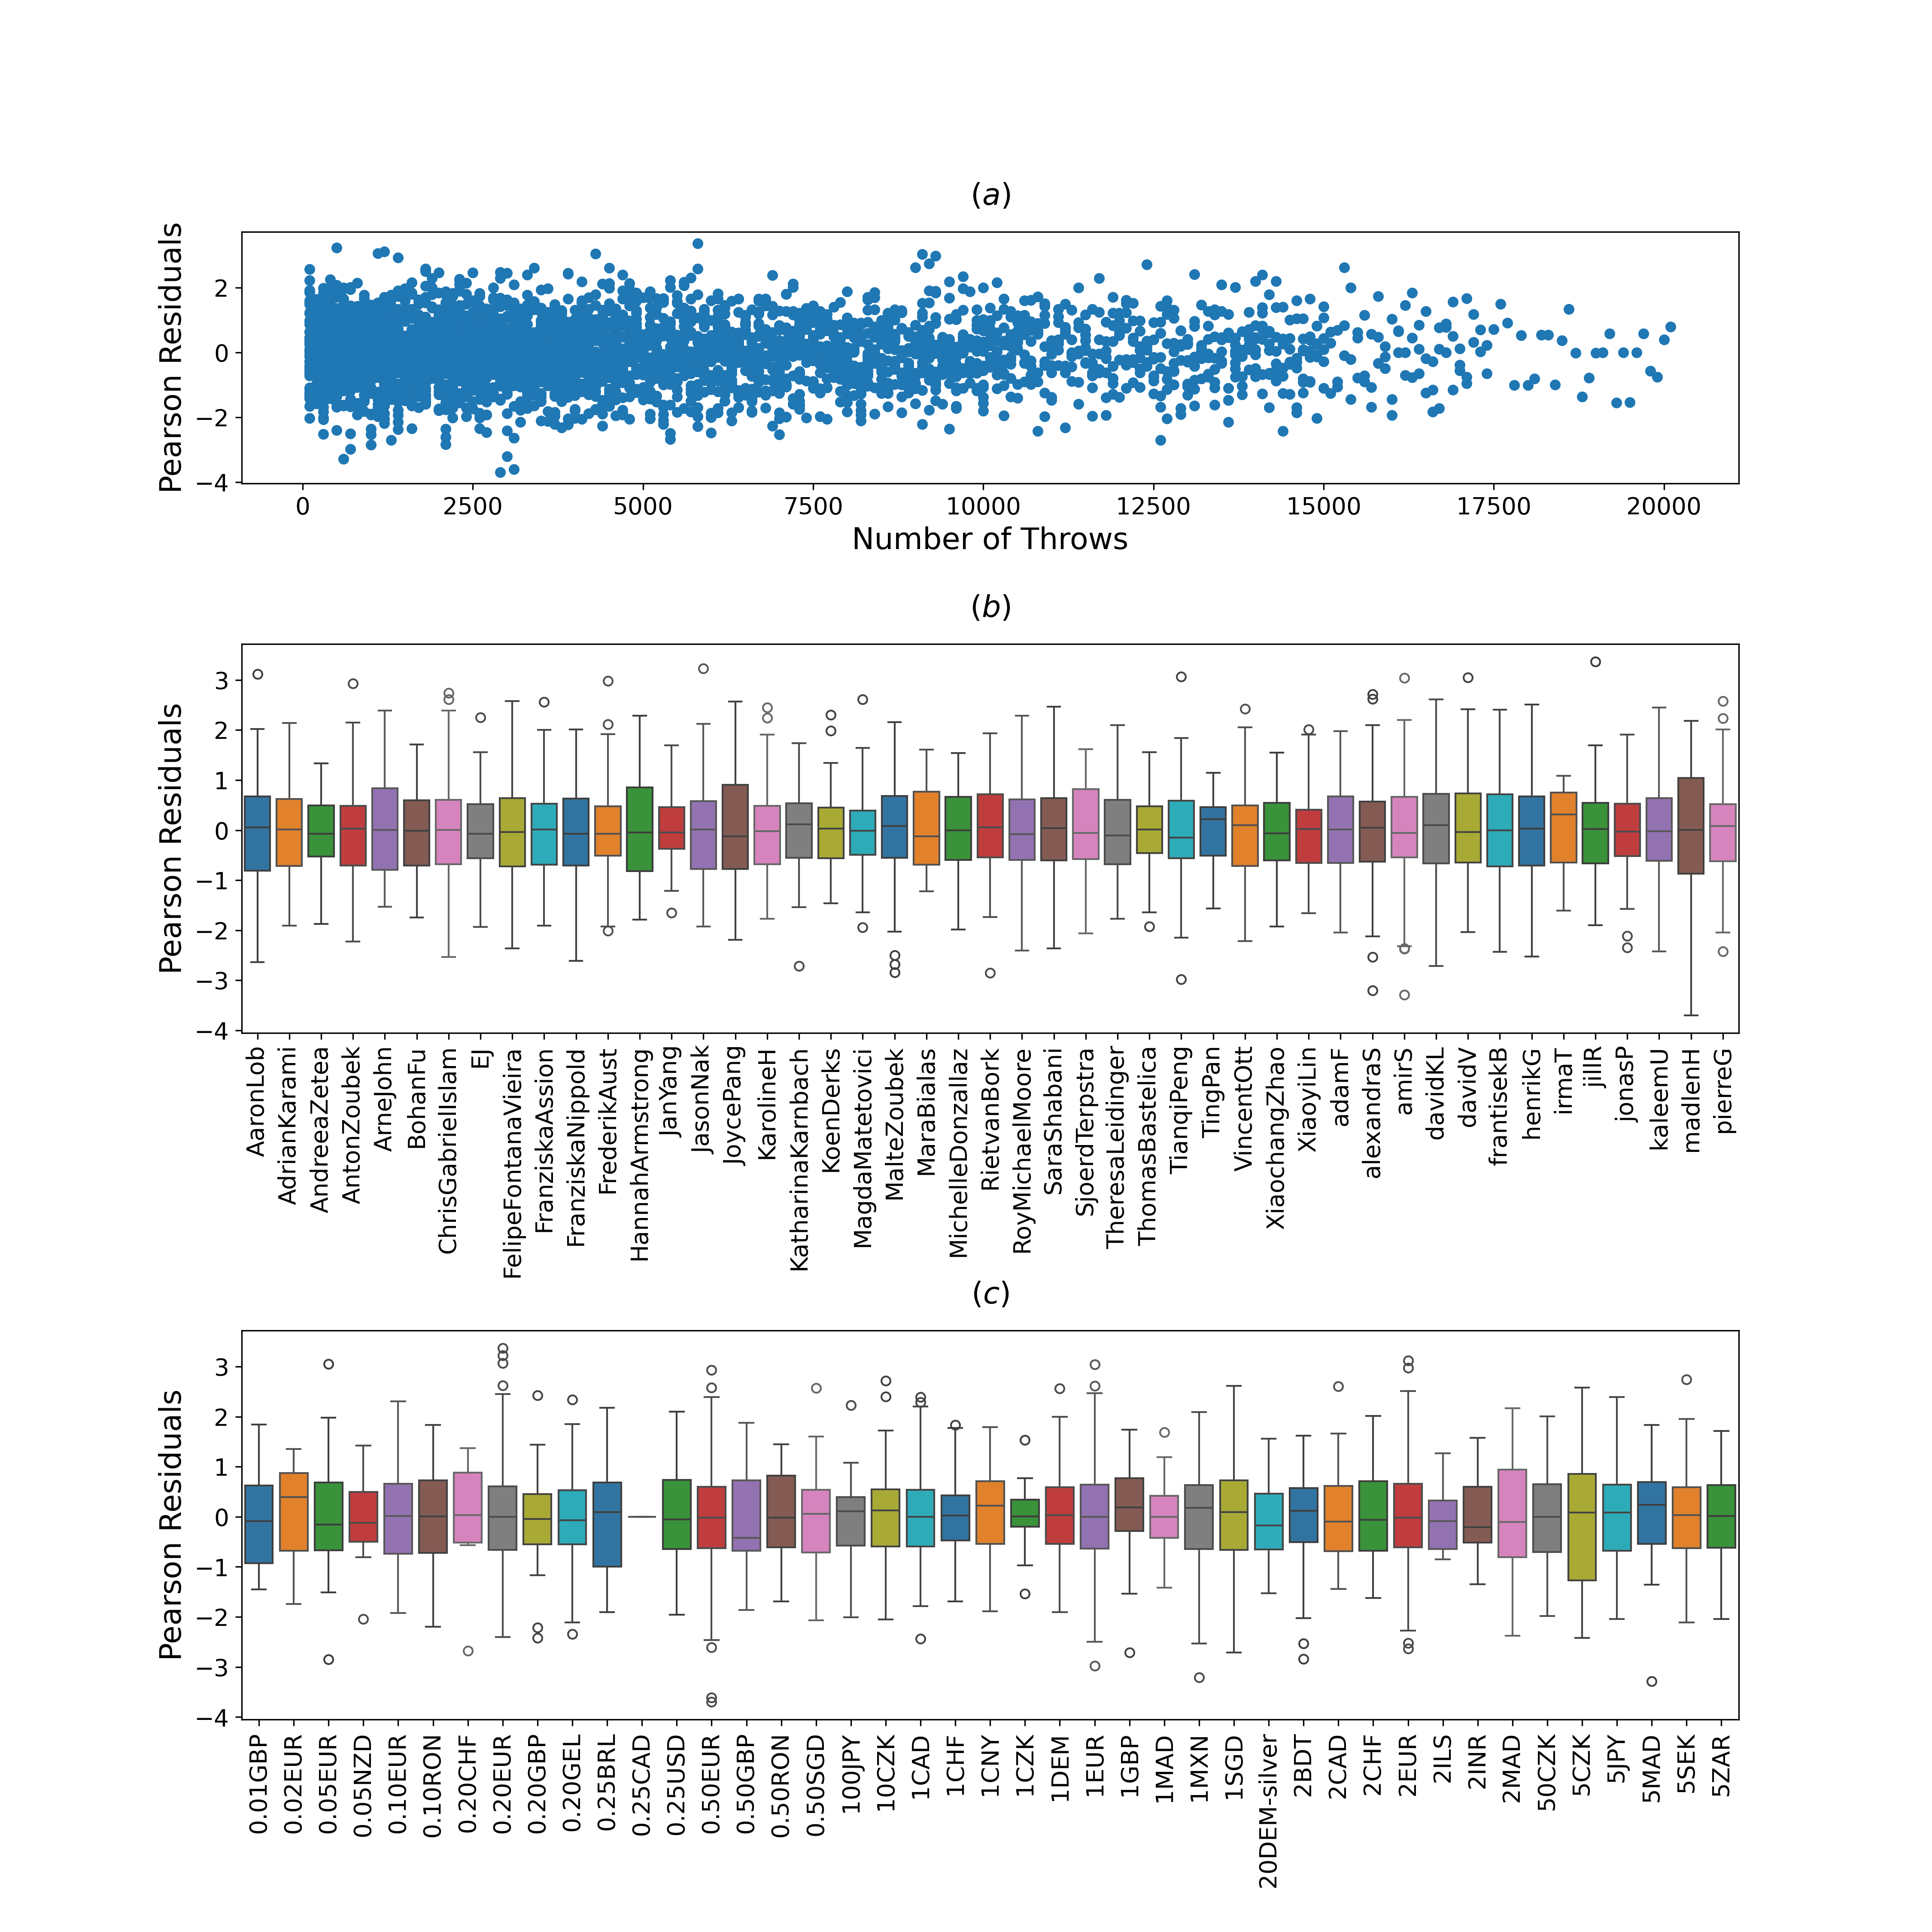
\includegraphics[width=0.85\textwidth]{wls_resid_vs_covariates.png}
				\caption{Pearson residuals as a function of covariates for the WLS \texttt{1+person+agg} model.}
				\label{fig:wls-diagnostic-time-coefs}
			\end{figure}

			Diagnostic plots for the model \texttt{1+person+agg} are reported in \ref{fig:wls-diagnostic} and \ref{fig:wls-diagnostic-time-coefs}. In \ref{fig:wls-diagnostic}, 1.5\% of the entries have a Cook's distance larger than the threshold fixed to $8/(n-2p)$. 
			\subsubsection{GLM Approach}
			In this section, instead of relying on an approximation to fit a weighted least squares models, we take into account the nature of the data by fitting a GLM. Indeed, given the aggregated data is binomial, using a binomial-response GLM is natural. 
			\begin{table}[htb]
				\centering
				% Top subtable
				\begin{subtable}{\textwidth}
					\centering
					\caption{Analysis of deviance of the GLM \texttt{1+person+agg+coin} model and AIC values.}
					\label{tab:glm-model-comparison}
					\begin{tabular}{lccc}
					\toprule
					Model & Deviance & AIC & Model DF \\
					\midrule
					\texttt{1} & 3942.13 & 187.84 & 0 \\
					\texttt{1+person} & 3676.20 & 13.91 & 46 \\
					\texttt{1+person+agg} & 3660.29 & 0.00 & 47 \\
					\texttt{1+person+agg+coin} & 3602.26 & 25.97 & 89 \\
					\bottomrule
					\end{tabular}
				\end{subtable}
				%\vspace{1em} % Optional vertical spacing

				\begin{subtable}{\textwidth}
					\centering
					\caption{LRTs for the GLM fitted models.}
					\label{tab:glm-lrt-comparison}
					\begin{tabular}{llc}
					\toprule
					Tested model & Restricted model & $p$-value \\
					\midrule
					\texttt{1+person} & \texttt{1} & 0.00e+00 \\
					\texttt{1+person+agg} & \texttt{1+person} & 6.63e-05 \\
					\texttt{1+person+agg+coin} & \texttt{1+person+agg} & 5.09e-02 \\
					\bottomrule
					\end{tabular}
				\end{subtable}
			\end{table}
			More specifically, we consider a Logit link as it leads to easily interpretable results, meaning we model $\mathbb{E}[y\mid x]=\exp\left(\sum_i \beta_i x_i\right)$ with binomial response distribution. We expect this to lead to more accurate results than the WLS approximation, especially for entries having $R/M\approx 1/2$ to a poor extent.

			As for the considered models, we follow what is done for the WLS approach. The only difference being in the interpretation of the coefficients and the fact that we omit the model with coins nested within people. Indeed, even the \texttt{0+person:coin} model did not give any signs of convergence after 100 IRLS iterations. We tried fitting it with BFGS, but did not succeed either as the hessian resulted to be singular. The analysis of deviance and LRTs for the models that converged are found in \ref{tab:glm-model-comparison} and \ref{tab:glm-lrt-comparison}.
			\begin{figure}[htb]
				\centering
				\includegraphics[width=0.8\textwidth]{glm_diagnostics.png}
				\caption{Main diagnostics for the GLM \texttt{1+person+agg} model.}
				\label{fig:glm-diagnostic}
			\end{figure}

			The diagnostic plots for the \texttt{1+person+agg} model are in \ref{fig:glm-diagnostic} and \ref{fig:dev-resid-vs-covariates}. 
			\begin{figure}[htb]
				\vspace{-1em}
				\centering
				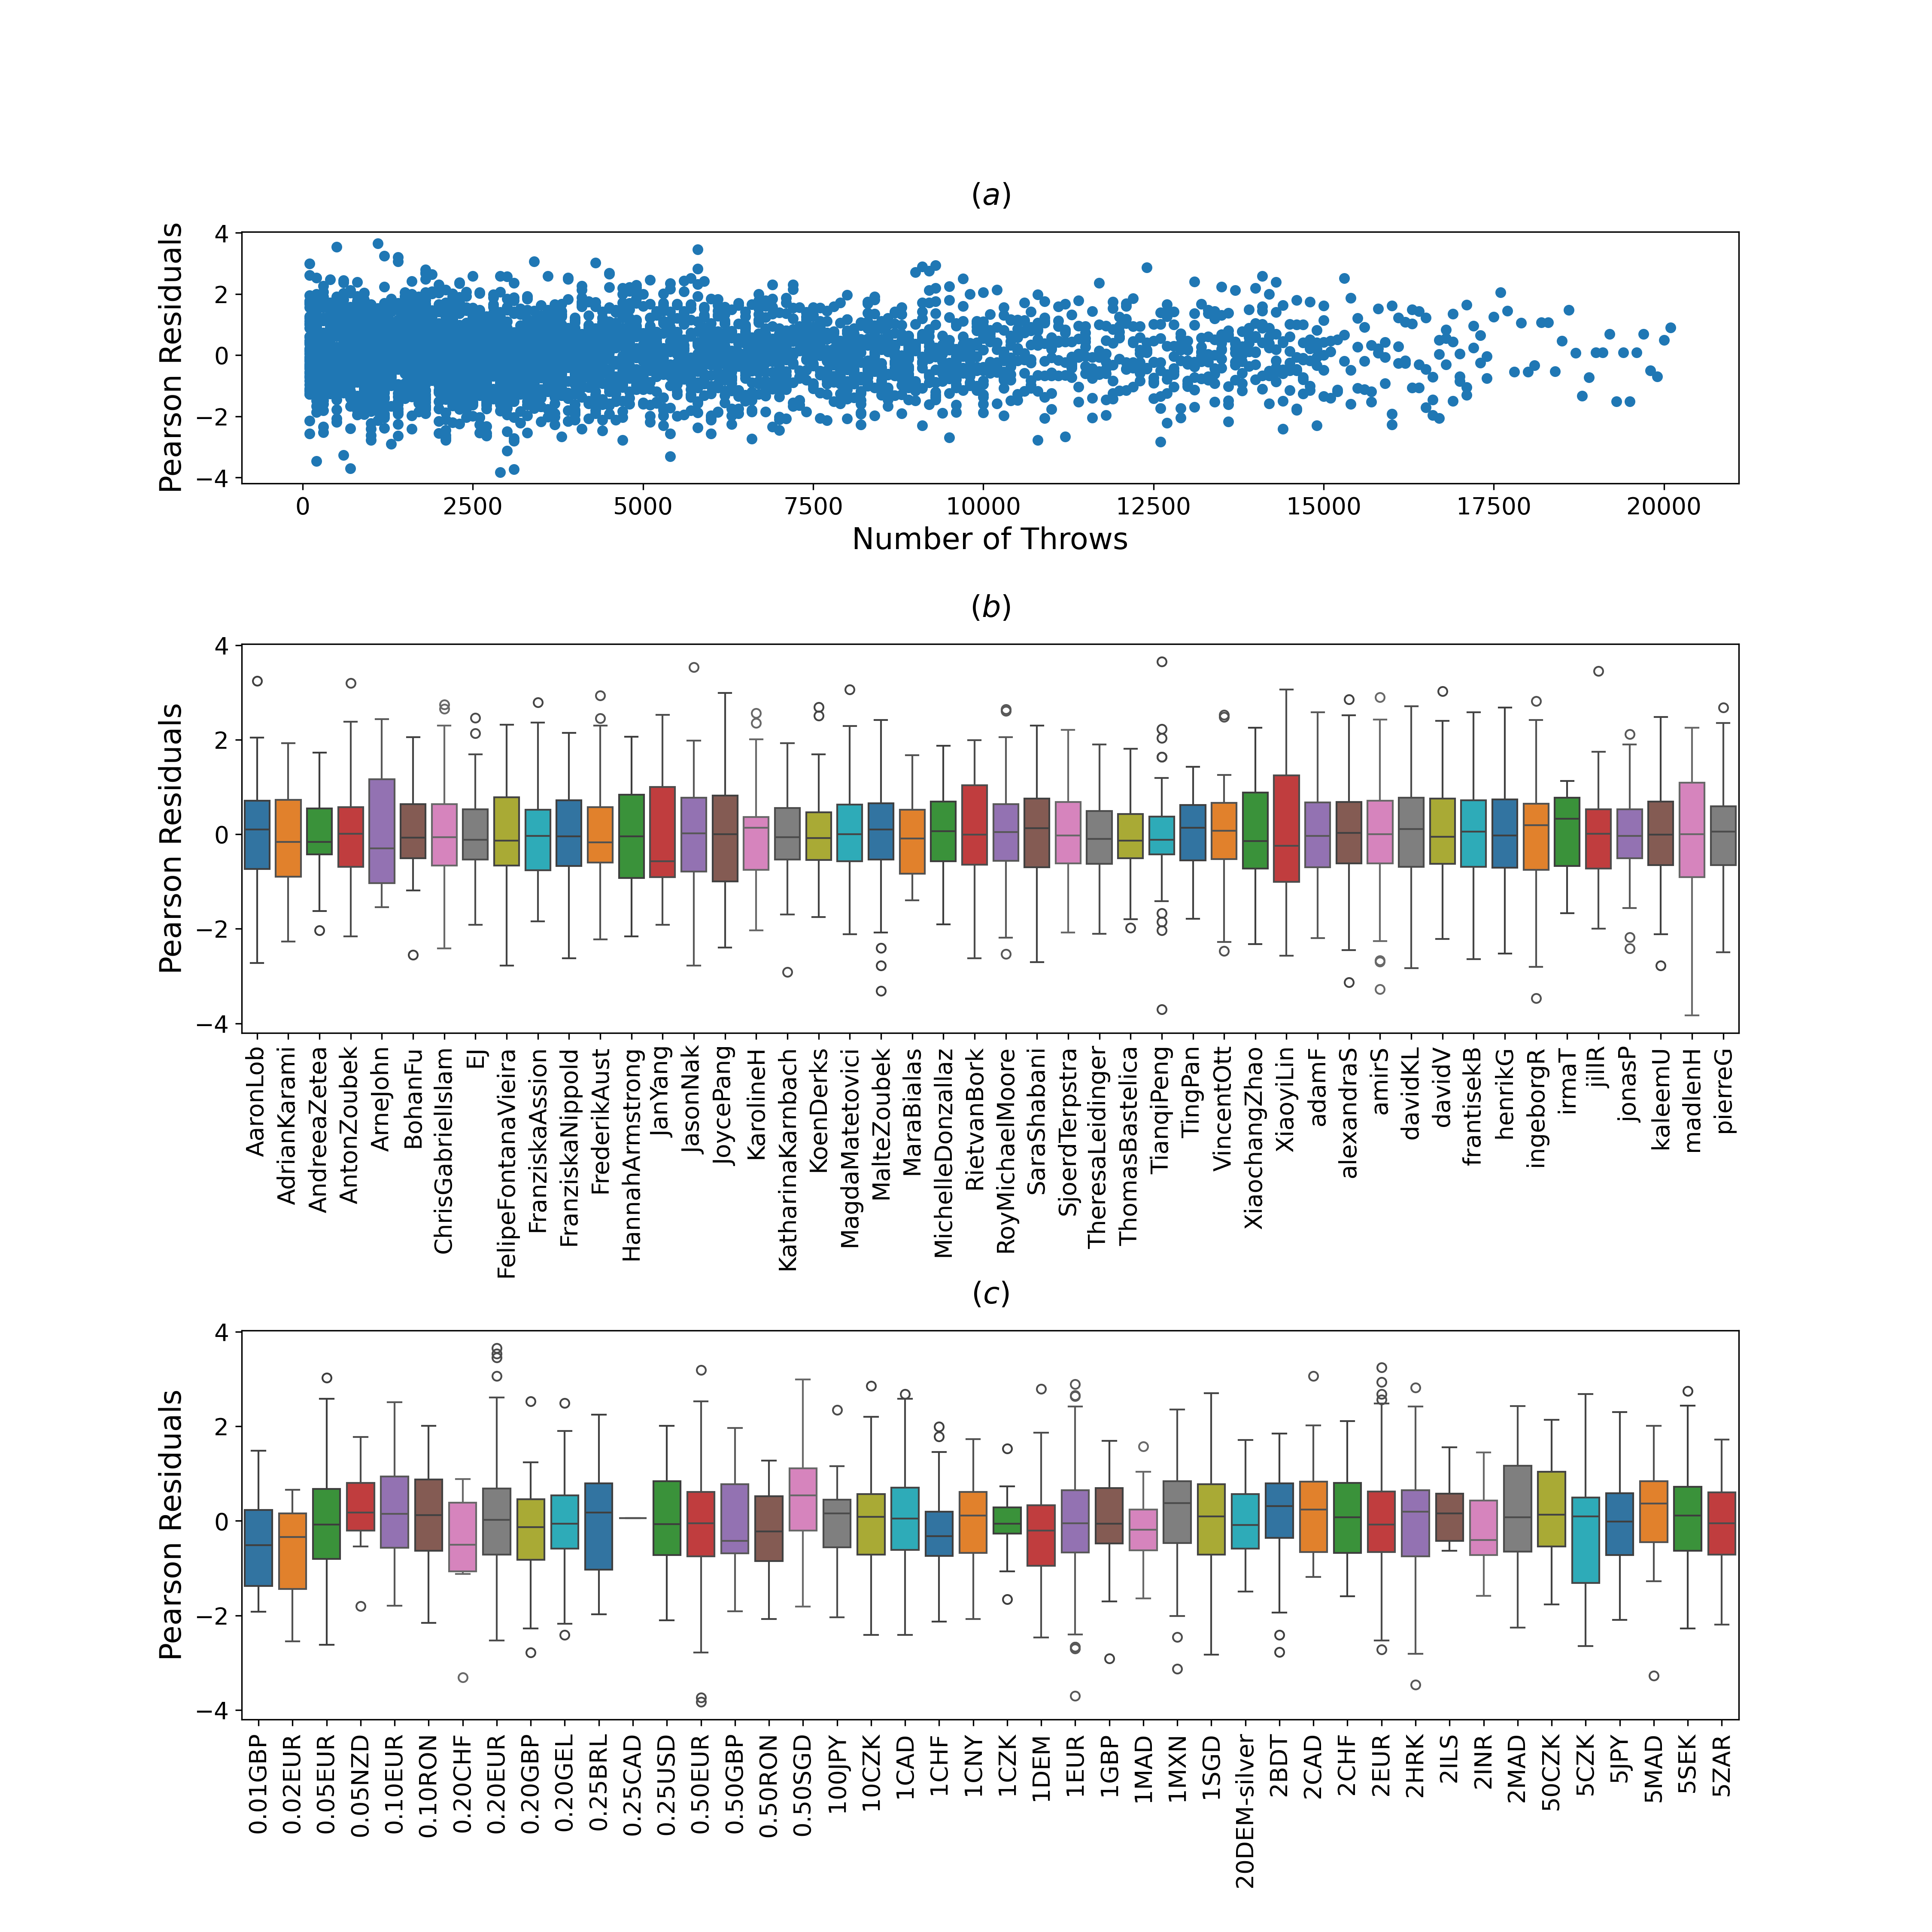
\includegraphics[width=0.85\textwidth]{glm_dev_resid_vs_covariates.png}
				\caption{Pearson residuals as a function of covariates for the GLM \texttt{1+person+agg} model.}
				\label{fig:dev-resid-vs-covariates}
			\end{figure}	
		%\newpage
		\subsection{Unusual Observations}
		In this section we present the results whose goal is to provide answers to questions such as ``are there unusual coins or people ?''. 
		\begin{figure}[h!]%{r}{0.6\textwidth}
			%\vspace{-4em}
			\centering
			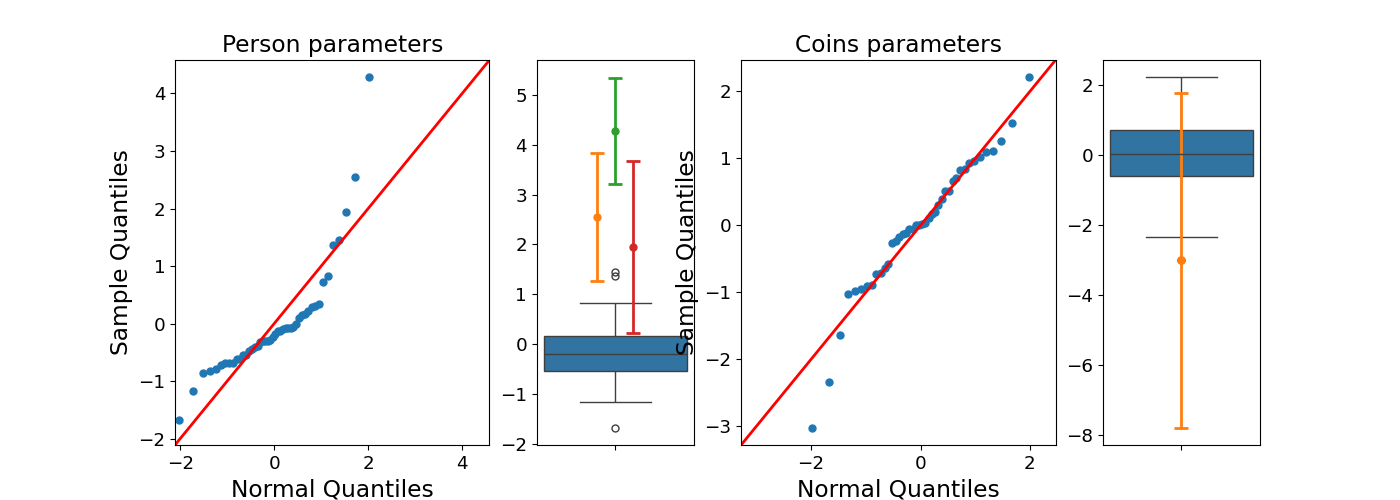
\includegraphics[width=0.9\textwidth]{glm_unusual_params.png}
			\caption{Distribution inspection for estimated parameters of the \texttt{1+person+coin} GLM model.}
			\label{fig:unusual-params}
		\end{figure}

		We considered ``unusual'' to mean that it seems to come from a different distribution compared to most of the other constituents of its population. We however recognise this is a broad question in principle, and could for example entail aspects such as ``do some people have really little same-side bias ?'' or ``are some people associated to surprisingly large (resp. small) variances between sequences ?''.
		%\newpage

		Given our interpretation of the question, we decided to compile normal QQ-plots for the coefficients, as well as box-plots to help identify outliers. The advantage of the box-plots is they allow for comparison under the assumption that the base distributions is not necessarily gaussian. 
		It also is advantageous in terms of the fact that it allows us to represent the uncertainty associated to the outliers, and therefore draw more accurate conclusions. Indeed, given the data is unbalanced, some outliers could be associated to much greater uncertainties, even as big as to make unwise to actually interpret them as outliers. 
		
		\begin{figure}[htb]
		%\begin{wrapfigure}[15]{r}{.6\textwidth}
			%\vspace{-1em}
			\centering
			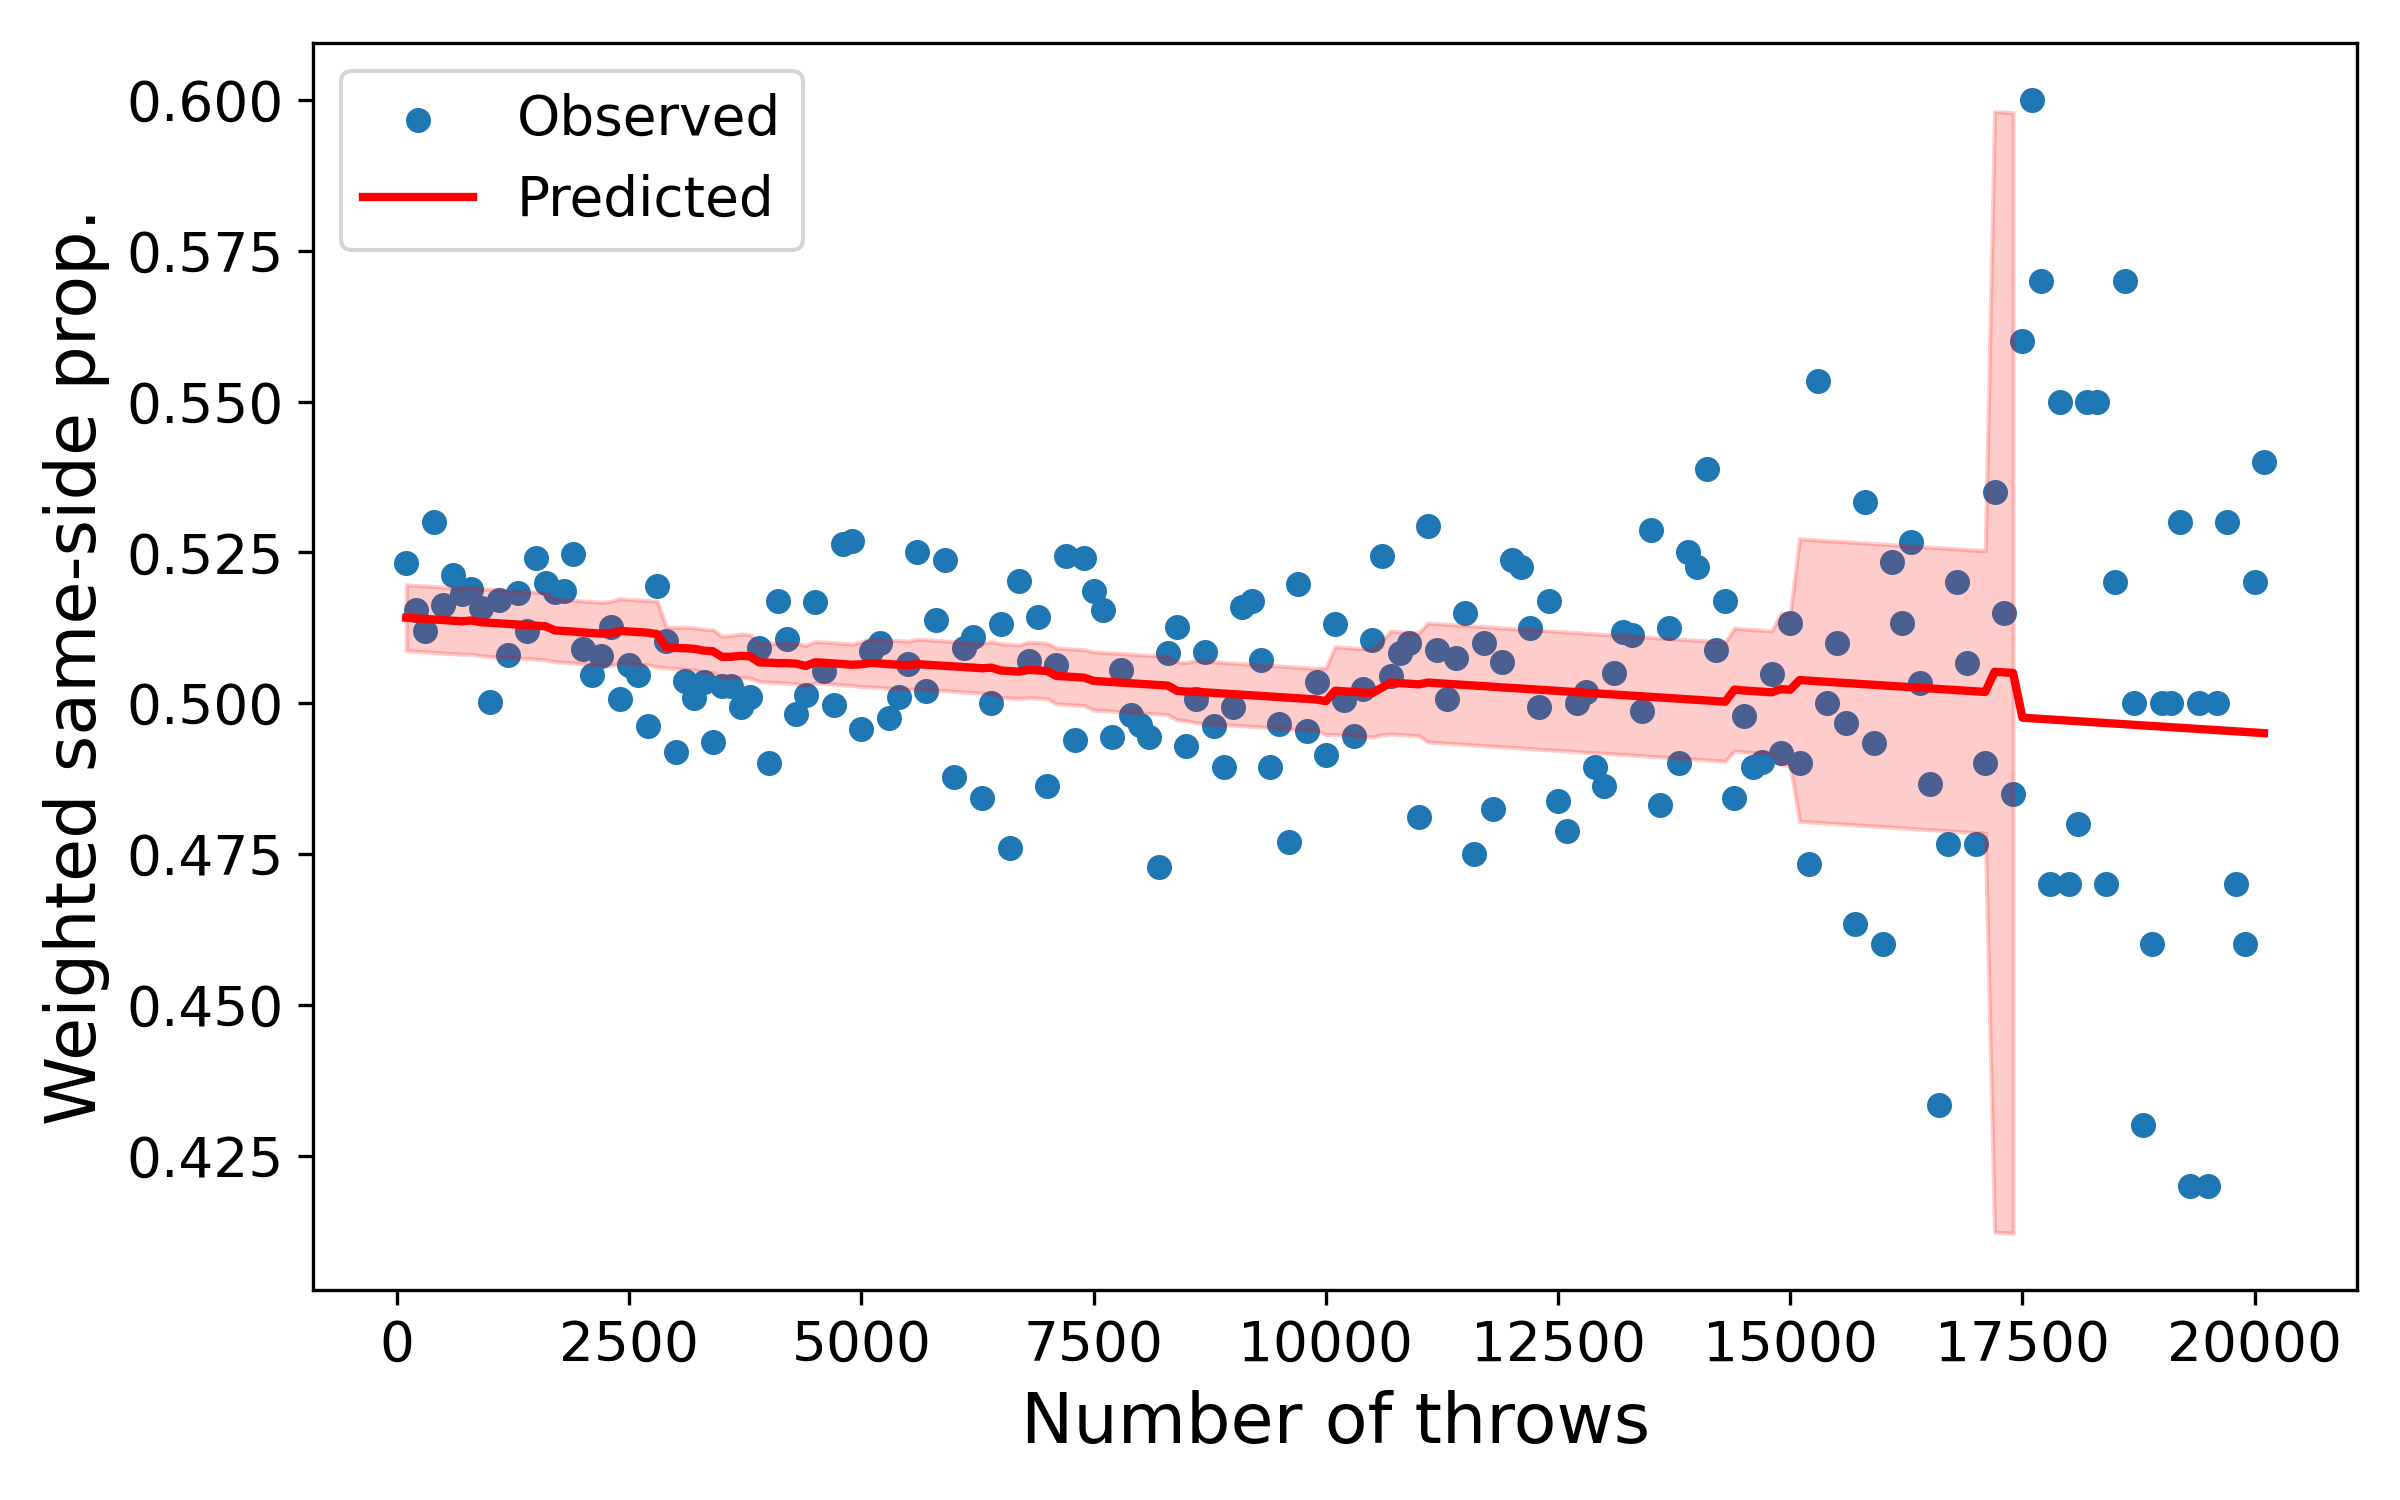
\includegraphics[width=.65\textwidth]{glm_learning_effects.png}
			\caption{Averaged same-side proportion as a function of cumulative number of throws (\texttt{100*agg}).}
			\label{fig:learning-effects}
		%\end{wrapfigure}
		\end{figure}
		The plots are found in \ref{fig:unusual-params}. Note we decided to include coins in the analysis because there could in principle still have been some that behaved differently from the rest (even if coins as a whole were found not to have much impact). 
		Another important detail is that we did not require people (resp. coins) to have been associated to multiple coins (resp. people) for them to be considered in this analysis. Indeed, since no evidence was found for coins nested within people, even the same-side behaviour of a person with a single coin should tell us something about that person's peculiarity.
		\subsection{Zoom on Learning Effects}
			We now give a closer look at the learning effects associated to the \texttt{agg} term in the model. We do this by representing the observed and predicted person-averaged same-side rate as a function of the number of throws preceeding the observation.  Note that the confidence interval on the prediction was derived in Monte Carlo fashion as the variance between people was found to be larger than that resulting from the uncertainty on the estimated coefficients. 
			The corresponding figure is \ref{fig:learning-effects}. 
		\subsection{Memory Effects}
			In this section we shift our focus to memory effects. We do so motivated by the fact that we deem it probable a priori that successive throws are more similar to each other than randomly selected ones. Indeed, one could imagine that after two same-side throws, the next could end being a same-side one too with a probability higher than the base rate (e.g. because of muscle memory effects). 
			\begin{table}[htb]
				\centering
				\caption{Analysis of deviance for GLM models with memory effects.}
				\label{tab:memory-model-comparison}
				\begin{tabular}{lccc}
				\toprule
				Model & Deviance & AIC & Model DF \\
				\midrule
				\texttt{1} & 474381.54 & 0.00 & 0 \\
				\texttt{1+hop1\_mem} & 474380.73 & 1.19 & 1 \\
				\texttt{1+hop1\_mem+hop2\_mem} & 474380.53 & 2.98 & 2 \\
				\bottomrule
				\end{tabular}
			\end{table}

			To test this we start by considering the data consisting of individual throw outcomes. To this, we add columns corresponding to same-side indicator variables, same-side indicator variables for the penultimate throw, and same-side indicator variables for the antepenultimate throw.
			To deal with the boundary effects between sequences of flips, we removed the two first entries of each sequence. 
			
			We then define the constant model \texttt{1}, the model including memory about the penultimate throw \texttt{1+hop1\_mem}, and the one including memory about the two previous throws \texttt{1+hop1\_mem+hop2\_mem}. The analysis of deviance associated to these models is found in \ref{tab:memory-model-comparison}. Given the uni-directionality of these results, no further analysis was made.  
	\section{Discussion}
		\subsection{Model Comparison}
		\subsubsection{WLS Approach}
		Examining table \ref{tab:WLS-AIC}, we see that there is a drop of AIC by 3 points per degree of freedom on average when adding the term \texttt{person} to the constant model, which strongly suggests the existence of differences between persons. Similarly, there is overwhelming evidence for time-dependence in the same-side bias. Indeed, the addition of the \text{agg} covariate allows a drop by 12 points in the AIC. When it comes to between-coin differences, the evidence is nowhere near as strong. Indeed, AIC increases by around 30 when compared to the \texttt{1+person+agg} model, reflecting clear overfitting.
		The same way, including the coefficients \texttt{person:coin} yields an increase in the AIC value of the model. 
		Overall, among the models reported in table \ref{tab:WLS-AIC}, the selection based on AIC leads to the model \texttt{1+person+agg}. 
		Likelihood ratio tests have also been reported (table \ref{tab:WLS-LRT}), leading to the same selected model. LRT results show that model \texttt{1+person} is prefered compared to the constant model \texttt{1}, and the model \texttt{1+person+agg} is prefered to the model \texttt{1+Cperson}. The last line in \ref{tab:WLS-LRT} shows that the model including the coins {1+person+agg+coin} is rejected when tested against the restricted model {1+person+agg}. 
		
		Interestingly, the model \texttt{1+person+agg+person:coin} tested against the model \texttt{1+person+agg} yields a p-value of 0.02 meaning that person coin interaction effects might still help in explaining part of the variance, even though the AIC-based selection rejected them.

		We now move to analysing the diagnostics of the selected model. Figures (a) and (b) in \ref{fig:wls-diagnostic} reveal healthy diagnostic plots. Indeed, the QQ plot shows a reasonably normal distriubtion of the residuals, with a small fat tail on the left for the smallest residuals. The plot (b) shows that no trend of residuals is observed with respect to the fitted values. 
		Plot (c) shows the cooks distance of each entry. Only a small fraction of entries (1.5\%) have a Cook's distance exceeding the threshold. Analyzing the 15 entries with the highest Cook's distances reveals that they all belong to individuals with relatively few throws. Ranking individuals in descending order by their number of throws shows that the 15 largest Cook's distances are associated with the 10 lowest-ranked (in terms of number of throws) individuals. According to the definition of Cook's distance, it increases with leverage. Leverage is higher for entries corresponding to individuals with fewer throws as it intuitively represents the "novelty" of the entry in terms of its position in the covariates space. This likely explains the large Cook's distances observed in these cases.
		Figure \ref{fig:wls-diagnostic-time-coefs} displays the Pearson residuals with respect to the covariates.
		Diagnostic plot (a) shows no discernible trend in Pearson residuals relative to the number of preceding throws, supporting the assumption of linearity.
		Diagnostic plot (b) indicates that residuals are fairly uniform across individuals, with means close to zero and no standout anomalies. Diagnostic plot (c) suggests no significant differences among coins, though it does reveal slightly greater variability, with some means deviating further from zero.

		\subsubsection{GLM Approach}
			We first consider the model comparison tables \ref{tab:glm-model-comparison} and \ref{tab:glm-lrt-comparison}. 
			Upon inspection of these, we see that the evidence for between-person variations is extremely strong. The deviance decreases by more than 5.5 points per degree of freedom on average, and the AIC drops by more than 170. Similarly as in the WLS approach, there is overwhelming evidence for time-dependence in the same-side bias. By itself, the term for example yields a deviance decrease of 15. A closer look at this contribution is given in the \ref{sec:disc-learning-effects}. Between-coin differences are not significant. Indeed, AIC increases by around 25 when compared to the \texttt{1+person+agg} model, reflecting overfitting. The associated LRT is around .05, meaning coin-effects might still help in explaining part of the deviance. A better evaluation of this could probably be obtained by considering a smaller scale, balanced-design study. Indeed, in the considered dataset, coin and time effects where aliased\footnote{Adding \texttt{coin} to the \texttt{1+person} model explained around 10 units of deviance more than when it was added in the \texttt{1+person+agg} model.}. This was a result of there being a strong time effect on same-side bias, and some coins being flipped many more times than others. 
			Given these elements, one would definitely prefer the \texttt{1+person+agg} model for prediction purposes.  

		We now move to analysing the diagnostics of the selected model. Looking at (a) and (b) of \ref{fig:glm-diagnostic}, we see that the residuals are for the most part appropriately normal and homoschedastic. Slight anomalies are observed in the QQ plot for the largest and smallest residuals, as well as for the residuals associated to the largest fitted same-side rate. Looking up the entries associated to the largest Cooks distances, we notice these are associated to sequences of throws where [TO FILL]
			\begin{itemize}
				\item best model (AIC vs LRT) + interpretation of significance (wobble )
				\item discussion of diagnostics 
				\item (rational of including agg, presentation of used residuals with assumptions)
				\item 
				\item comparison with WLS (coefs ?? accuracy ?)
			\end{itemize}

		\subsection{Unusual Observations}
			Looking at \ref{fig:unusual-persons} and \ref{fig:unusual-coins}, we immediately notice they look really different. Indeed, in the case of coins, the parameters align quite well on the QQ plot, showing that a gaussian could be a good match. In the box-plot, there is a single outlier (associated to 0.02 EUR) and it is not significant. In the person case however : the QQ plot displays really poor fit and  many outliers are present. The most significant are (in order) JanYang, TianqiPeng and adamF. 

			In general, the observed variation in the parameter uncertainties confirm our approach accounting for uncertainty was worth our time. 
			%[COULD ADD EXAMPLE OF IMPACT in terms of flips]
			%\item  person distribution being asymmetric (could be a thing ?)
		\subsection{Zoom on Learning Effects}\label{sec:disc-learning-effects}
			Analysing \ref{fig:learning-effects}, we see that the averaged same-side rate seems to start at a value around 51\%, and then decreases to reach values closer to 50\%. The observed uncertainty/spread can however no be neglected, given the limited number of people involved in the study. 
			
			This would be consistent with the fact that the physical model [CITATION NEEDED] predicts a same-side bias due to the ``wobble'' in people's throws. Indeed, we can imagine that with practice, participants progressively reduce the amount of ``wobble'', until they reach perfect throw, for which there is no bias. 

			As for the type of dependence, the simple linear term at the exponential seems to provide a good fit.  
		\subsection{Memory Effects}
		Looking at \ref{tab:memory-model-comparison}, we see there is no support in favour of memory effects relative to the constant model. The deviance decreases by around .8 due to the introduction of the penultimate throw memory and only a further .2 when including memory of the antepenultimate throw. Another factor that shows this is the increase by $>$1 and $\approx 3$ respectively in AIC compared to the constant model.
		The fact that memory about antepenultimate outcome seems to matter even less than memory about the penultimate outcome does make nonetheless intuitive sense. 

		This (non-) finding can in itself be regarded as reassuring in a way. Specifically, it might contribute to rule out concerns of the authors of the original paper regarding the potential same-side bias induced by participants knowing about the goal of the study. Indeed it seems far-fetched that someone could bias their throws without relying on muscle memory. 
	\section{Conclusion}
	\section*{Acknowledgements}
		\paragraph{Tara:}
		I personally use Github Copilot for coding purposes, as it can gain me some time by auto-completing lines. I however never keep lines I don't understand or find not relevant. I also sometimes used Chat GPT to brainstorm ideas related to some problems I faced and did not have the right resources to tackle. In these cases I still kept a critical mindset and dug deeper in the directions that seemed promising.
		\paragraph{Rayan:}
		[CETTE PARTIE ETAIT CELLE DE AMAL POUR LE RAPPORT DE HPC, ADAPTE LA ;)]
		ChatGPT was used to refine the English, generate code for the plots. Additionally, ChatGPT provided comments throughout the report and to the code to enhance readability.
	\section*{Reproducibility}
		In the spirit of making our analysis reproducible, we created an \texttt{environment.yml} file containing the needed packages (with their versions) so that the appropriate virtual environment can be readily created. We also used \texttt{git} to do version control. This allows us to make the project repository public (after the submission deadline of course) for people to have easy and complete access to our work. 
	\section*{References}
		\noindent[1] F. Bartoš et al., `Fair coins tend to land on the same side they started: Evidence from 350,757 flips', Jun. 02, 2024, arXiv: arXiv:2310.04153. doi: 10.48550/arXiv.2310.04153.
		\newline[2] Anthony Davison, `Regression Methods'. Accessed: Jan. 07, 2025. [Online]. Available: \url{https://moodle.epfl.ch/pluginfile.php/3309119/mod_resource/content/6/RMNotes.pdf}
		\newline[3] nzcoops, `Anova - Type I/II/III SS explained - R-bloggers'. Accessed: Jan. 07, 2025. [Online]. Available: \newline\url{https://www.r-bloggers.com/2011/03/anova-\%e2\%80\%93-type-iiiiii-ss-explained/} 
		\newline[4] Ø. Langsrud, `ANOVA for unbalanced data: Use Type II instead of Type III sums of squares', Statistics and Computing, vol. 13, no. 2, pp. 163--167, Apr. 2003, doi: 10. 1023/A:1023260610025.
	%\appendix
	%	\section{Runtime Estimation}\label{appendix:runtime_estimation}
%%%
\end{document} 